In this chapter the theoretical foundations for the development of this project are presented, creating a solid groundwork for the design and implementation process.

%\section{Concurrency}

%\section{Threads versus Processes}

%\section{Signals}

\section{Communication Protocols}
% assim tudo misturado aqui dentro?
\subsection{LoRaWAN}

\subsection{SPI}
\subsection{I2C}

\subsection{CSI}
%by way of a 15 Pin Ribbon Cable, to the dedicated 15-pin MIPI Camera Serial Interface (CSI), which was designed especially for interfacing to cameras. The CSI bus is capable of extremely high data rates, and it exclusively carries pixel data to the BCM2835 processor. 

\subsection{TCP-IP}
\subsection{HTTP}
\subsection{MQTT}

%********************************* DAEMONS *************************
\clearpage
\section{Daemons}
A daemon is a process that runs in the background and has no controlling terminal. The lack of a controlling terminal ensures that the kernel never automatically generates any job-control or terminal-related signals (such as SIGINT, SIGTSTP, and SIGHUP) for a daemon. \cite{linux_progr_interface}

A daemon is often created at system startup and runs until the system is shut down, being used to carry out specific tasks. It is a convention (not universally observed) that daemons have names ending with the letter d (example: \textit{httpd}, \textit{sshd}). 

Each process belongs to a process group, and the process group can contain one or more processes. There is a process leader in the process group, the \ac{pid} of the leader is the \ac{pgid}. More than one process group constitutes a "session". The process that establishes the session is the lead process for the session, and the \ac{pid} of the leader is the \ac{sid} of the session. Each process group in a session is called a "job". The meaning of a session is that multiple jobs can be controlled through one terminal, one foreground operation and the other running in the background. \cite{daemons}\newline

To become a daemon, a program performs the following steps:
\begin{enumerate}
	\item Perform a \textit{fork()}, after which the parent exits and the child continues.
	\item The  child  process  calls  \textit{setsid()} to  start  a  new  session  and  free itself of any association with a controlling terminal.
	\item Clear the process umask to ensure that, when the daemon creates files and directories, they have the requested permissions. (\textit{umask()})
	\item Change the process’s current working directory, typically to the root directory (\textit{chdir('/')}). This is necessary because a daemon usually runs until system shutdown, and if the daemon’s current working directory is on a file system other than the one containing '/', then that file system can’t be unmounted.
	\item Close  all  open file descriptors that the daemon has inherited  from its parent. (\textit{close()}) (A  daemon  may  need  to  keep  certain  inherited  file  descriptors  open,  so  this step  is  optional,  or  open  to  variation.)
\end{enumerate}

Since a daemon has no controlling terminal, the  \textit{syslog}  facility  provides  a  convenient  way  for  daemons  (and  other  applications)  to  log  error  and  other  messages  to  a  central  location.  These  messages  are processed by the \textit{syslogd} daemon, which redistributes the messages according to the dictates  of  the  syslogd.conf  configuration  file. 

Where appropriate, daemons should correctly handle the arrival of the SIGTERM and SIGHUP  signals. The  SIGTERM signal  should  result  in  an  orderly  shutdown  of  the daemon, while the SIGHUP signal provides a way to trigger the daemon to reinitialize itself by rereading its configuration file and reopening any log files it may be using.

%********************************* DEVICE DRIVERS *************************
\clearpage
\section{Device Drivers}
System memory in Linux can be divided into two distinct regions: kernel space and user space. Kernel space is where the kernel (the core of the operating system) executes and provides its services. User space is that set of memory locations in which user processes (everything other than the kernel) run. One of the roles of the kernel is to manage individual user processes within this space and to prevent them from interfering with each other. User processes can access kernel space only through the use of system calls, which are requests in a Unix-like operating system by an active process for a service performed by the kernel, such as input/output or process creation. \cite{kernel_space}

A device driver is a set of functions and data, in the kernel, that make the interface with an external I/O device. They are distinct “black boxes” that make a particular piece of hardware respond to a well-defined internal programming interface, hiding completely the details of how the device works. Devices  are  represented  by  entries  in  the  /dev  directory, being considered regular files.  Each  device  has  a  corresponding device driver, which implements a standard set of operations, including those  corresponding  to  the  \textit{open()},  \textit{read()}, \textit{ write()},  and  \textit{close()}  system  calls. \cite{linux_dev_drivers}

User activities are performed by means of a set of standardized calls that are independent of the specific driver. So the role of the device driver is to map those calls to device-specific operations that act on real hardware. Linux kernel offers a set of functions to the user space for the interaction with hardware, as one can see in the table \ref{table:device_driver}, in "User Functions". In the kernel space, Linux offers a set of functions that interact directly with the hardware and allows data transfer between kernel space and user space, as shown in "Kernel Functions".

\begin{table}[H]
	\centering
	\resizebox{\columnwidth}{!}
	{
		\begin{tabular}{|m{4cm}|m{3.5cm}|m{5cm}|}
			\hline
			\textbf{Event} & \textbf{User Functions} & \textbf{Kernel Functions}
			\\\hline\hline
			Load module & insmod & module\_init()
			\\\hline
			Remove module & rmmod & module\_exit()
			\\\hline
			Open module & fopen() & file\_operations: open
			\\\hline
			Read from device & fread() & file\_operations: read
			\\\hline
			Write to device & fwrite() & file\_operations: write
			\\\hline
			Close module & fclose() & file\_operations: close
			\\\hline
		\end{tabular}
	}
	\caption{Interface between an event, it's user function, and the kernel function called.}
	\label{table:device_driver}
\end{table}

When the kernel recognizes that a certain action were requested to a device, it calls an appropriate function from the driver, and transfers the process control from the user to the driver function. After the driver function ends its execution, it gives the control back to the user space process.

To associate the normal files to the kernel mode, the Linux system uses the major number and the minor number. Major number identifies the driver associated to the device and is normally used by Linux system to map I/O requests to driver code. Minor number is dedicated to internal use and it is used by kernel to determine exactly which device was reference. To do the association, it should be created a file or node in /dev directory, (calling \textit{mknod} as root user) that will be used to access the driver.

Linux supports three types of hardware devices: character, block and network device, being the character and block devices the most important. Character devices communicate directly with the user space program, so no buffer is required, for example the system’s serial ports. Block devices are accessed by the user space program by a system buffer, and can only be written and read from in multiples of the block size, typically 512 bytes. \cite{linux_progr_interface}

%********************************* IMAGE PROCESSING *************************
\clearpage
\section{Image Processing}
%Basically, an image is a two-dimensional array of pixels, so it can be represented in an cartesian coordinate system. 

Image processing consists of several techniques and methods used to manipulate images on a computer. The image processing helps improving the stored digital information, automate working with images and optimize image manipulation leading to efficient storage and transmission. Nowadays, image processing has many applications, like filtering images in editing apps and social media, medical technology, computer vision (objects identification, for example), pattern recognition, video processing and more. In this project, the image processing application is the computer vision, to detect available parking spots in the streets, using a camera.

In order to identify parking spots, one needs to find its outlines. The Canny Edge Detection \cite{canny} algorithm is a popular edge detection algorithm, and can be used to detect the parking spots outlines, providing an edge image. The canny edge detection is a multi-stage algorithm that goes through the stages: Noise reduction, Sobel Filtering, Non-maximum Suppression and Hysteresis Thresholding.

\myparagraph{Noise reduction}
The edge detection algorithm is sensible to noise in the image, so the first step is to remove the noise in the image using a 5x5 Gaussian filter. In figure \ref{fig:gaussian} one can see the results of the gaussian filter 5x5. 

\begin{figure}[H]
	\centering
	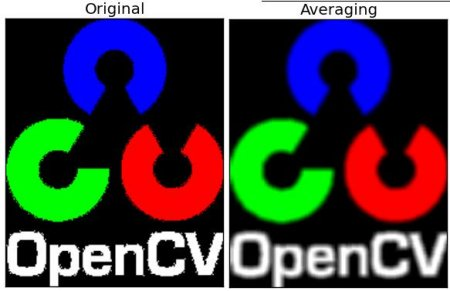
\includegraphics[width=.6\textwidth]{08theory/gaussian}
	\caption{Gaussian Filter Results.}
	\label{fig:gaussian}
\end{figure}

\myparagraph{Sobel Filtering}
Sobel filtering is an algorithm that finds intensity gradients on the image. This filter is applied in both horizontal and vertical direction, allowing to find the edge gradient and direction for each pixel. Figure \ref{fig:sobel}, shows the sobel filtering results.

\begin{figure}[H]
	\centering
	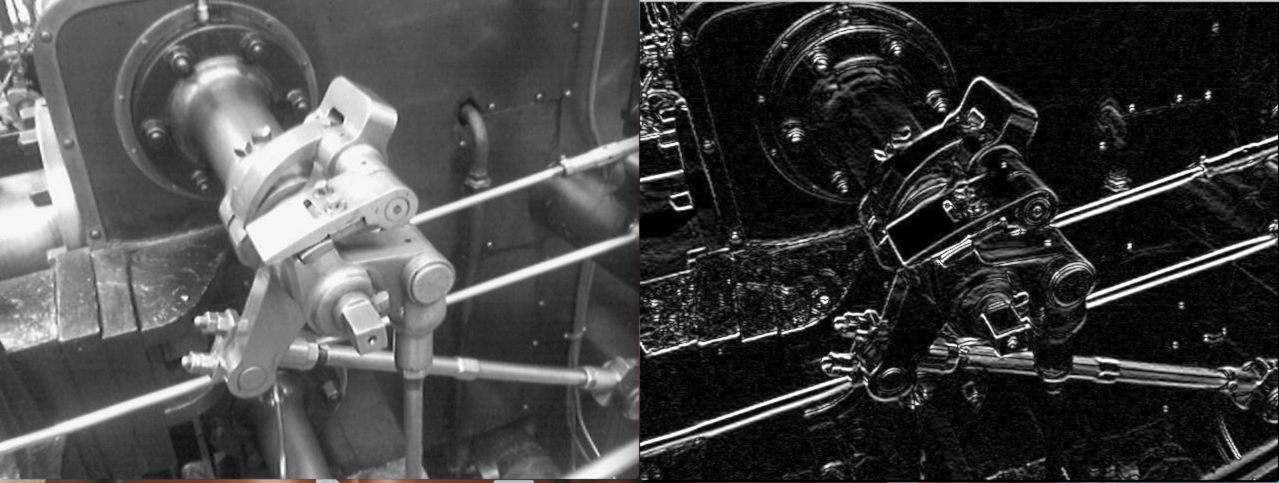
\includegraphics[width=.75\textwidth]{08theory/sobel}
	\caption{Sobel Filter Results.}
	\label{fig:sobel}
\end{figure}

\myparagraph{Non-maximum Suppression}
The non-maximum suppression algorithm does a full scan of the image in order to remove any unwanted pixels, that is, the pixels that don't constitute the edges of the image. In figure \ref{fig:nms}, one can see the non-maximum suppression algorithm. The point A is on the edge and the point B and C are in gradient directions. This algorithm suppresses the points B and C (put their pixel to 0) if they aren't a local maximum. If they are a local maximum, they are considered for the next stage as well as the point A.

\begin{figure}[H]
	\centering
	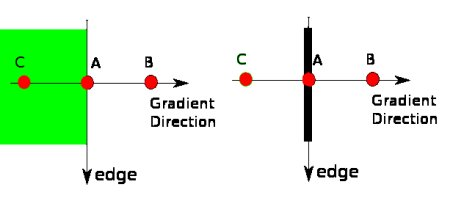
\includegraphics[width=.75\textwidth]{08theory/nms}
	\caption{Non-maximum Suppression Algorithm.}
	\label{fig:nms}
\end{figure}

\myparagraph{Hysteresis Thresholding}
This stage decides which edges considered until this point are really edges. This algorithm defines two threshold values, \textit{minVal} and \textit{maxVal}, in figure \ref{fig:hys_thr}. The edges that have an intensity gradient higher than \textit{maxVal} are considered edges and the edges that have lower intensity gradient than \textit{minValue}, aren't considered edges. The points with intensity gradient between this values are considered edges when they are connected to other edges with intensity gradient higher than \textit{maxVal} threshold value (the case of point C), and considered non-edges when they are not connected with other points with high intensity gradient value (the case of point B). 

\begin{figure}[H]
	\centering
	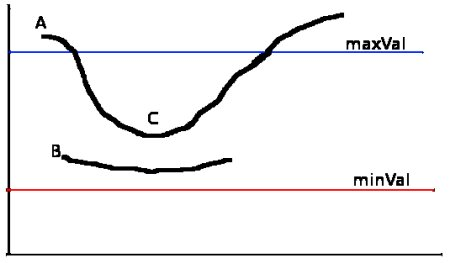
\includegraphics[width=.5\textwidth]{08theory/hys_thr}
	\caption{Hysteresis Thresholding Algorithm.}
	\label{fig:hys_thr}
\end{figure}

This algorithm, the Canny Edge Detection, allows the image processing algorithm to have only the strong edges of an image, being the final result represented in figure \ref{fig:canny}.

\begin{figure}[H]
	\centering
	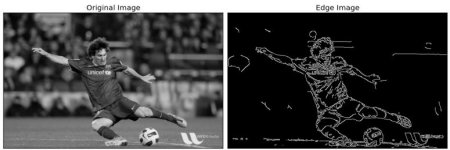
\includegraphics[width=.75\textwidth]{08theory/canny}
	\caption{Canny Edge Detection Result.}
	\label{fig:canny}
\end{figure}

\clearpage
\myparagraph{Hough Line Transform}

After detecting the edges of the image, one needs to take the processed image and use Hough Line Transform, which is an algorithm used to detect straight lines in an image. \cite{hough} 

Knowing that a parking spot is delimited by straight line edges, this algorithm provides the extreme coordinates of the parking spot outline. With the parking spots coordinates, one can make a parking map and knows where there are parking spots to after identify if the spot is occupied or not.

\begin{figure}[H]
	\centering
	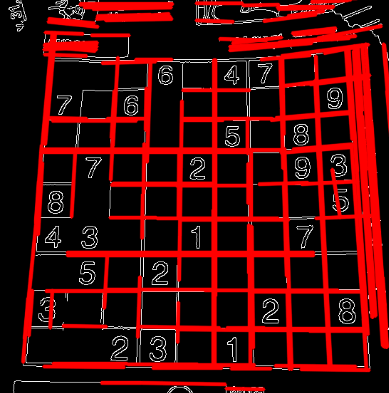
\includegraphics[width=.5\textwidth]{08theory/hough}
	\caption{Hough Line Transform Result.}
	\label{fig:hough}
\end{figure}

\myparagraph{Parking Spots Occupancy}

With the parking spots mapping, it is possible to identify the parking spots status. One can do that in three different ways:

\begin{itemize}
	\item Check if the pixel colour of the spot aligns with the colour of an empty parking spot;
	\item Detect all cars and check if the car's location match with the parking spot coordinates;
	\item Take two pictures of the parking spots: one available and other occupied. The occupied and empty spots look very different, making it easy to identify the parking spot status.
\end{itemize}

\myparagraph{Pixel Colour Change}

To detect if a car is in the parking spot, one can see the change in the pixel colour of the spot. It can be done by calculating the spot pixel colours average and comparing it to the empty spot pixel colour average. If the average calculated is higher or lower than a pre-defined value, then the parking spot is occupied.

\myparagraph{Cascade Classifier Training}

The second way to identify the parking spot status is using a Cascade Classifier Training \cite{cascade}. This is divided into two major stages: training and detection. For training it is needed a set of samples, negatives and positives. The negative samples correspond to non-object images and the positive samples correspond to images with detected objects. Then it is required to create a positive vector using an OpenCV utility that gathers all the positives. The last step is to train the cascade, creating a \ac{xml} file that can be used to detect objects of a frame.
